\section{Model Evaluation}
\label{sec-evaluation}
% \begin{figure*}[!t]
%     \centering
%     \subfigure[Traditional Lens]{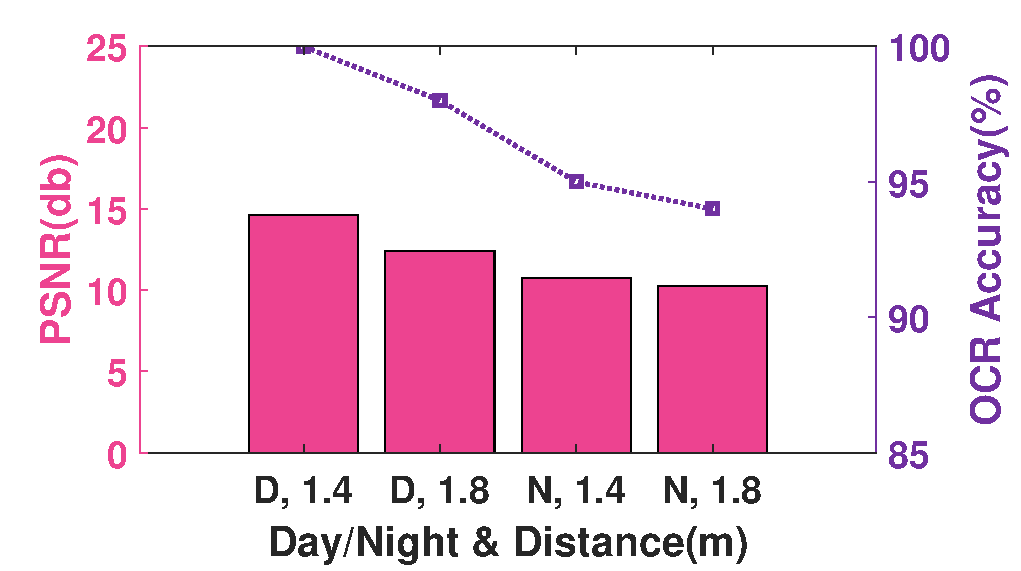
\includegraphics[width=0.24\textwidth]{./pic/data_1.pdf}\label{fig-control-1}}
%     \subfigure[Optical Lens]{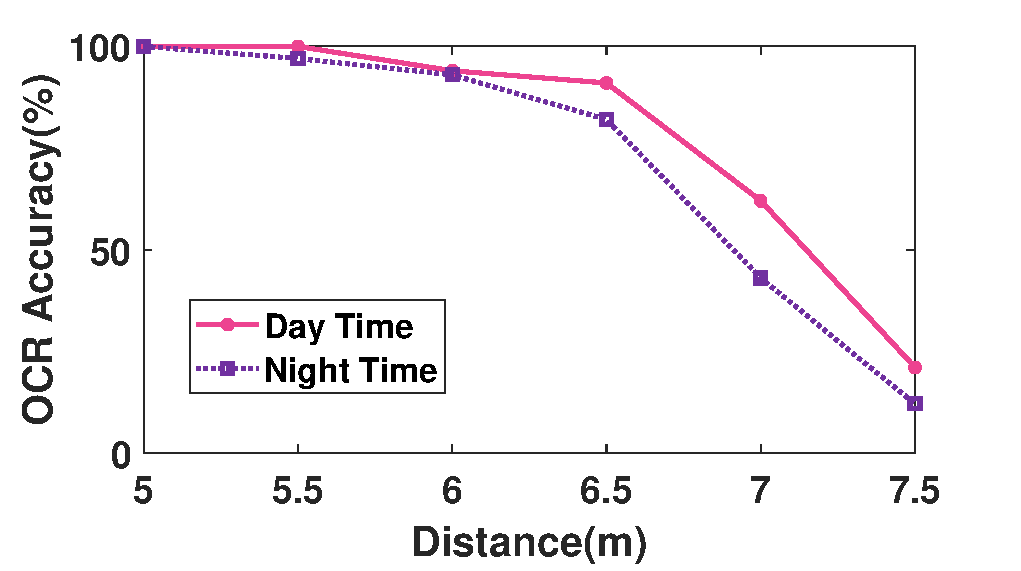
\includegraphics[width=0.24\textwidth]{./pic/data_1_2.pdf}\label{fig-control-2}}
%     \subfigure[Traditional Lens]{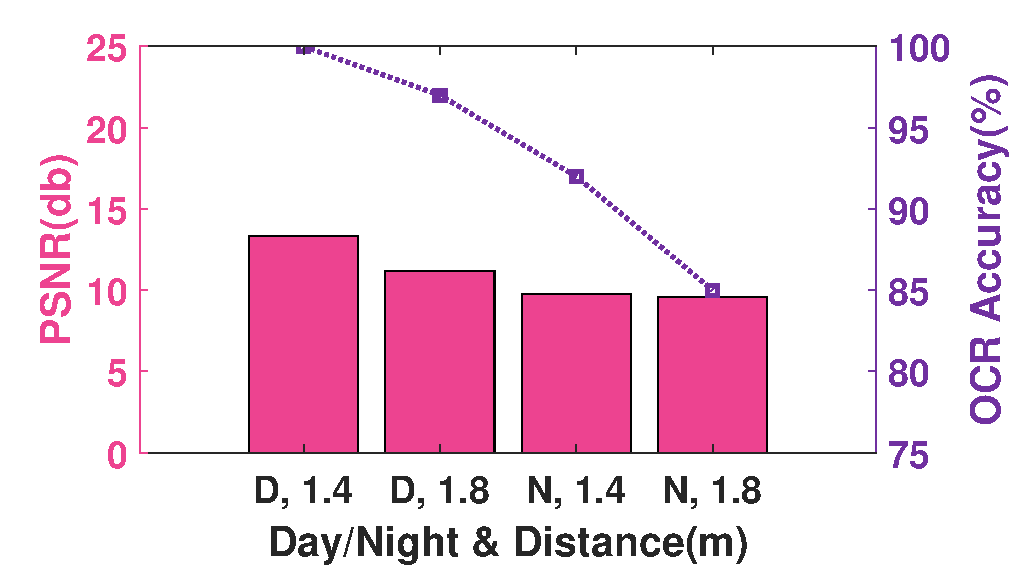
\includegraphics[width=0.24\textwidth]{./pic/data_2.pdf}\label{fig-random-1}}
%     \subfigure[Optical Lens]{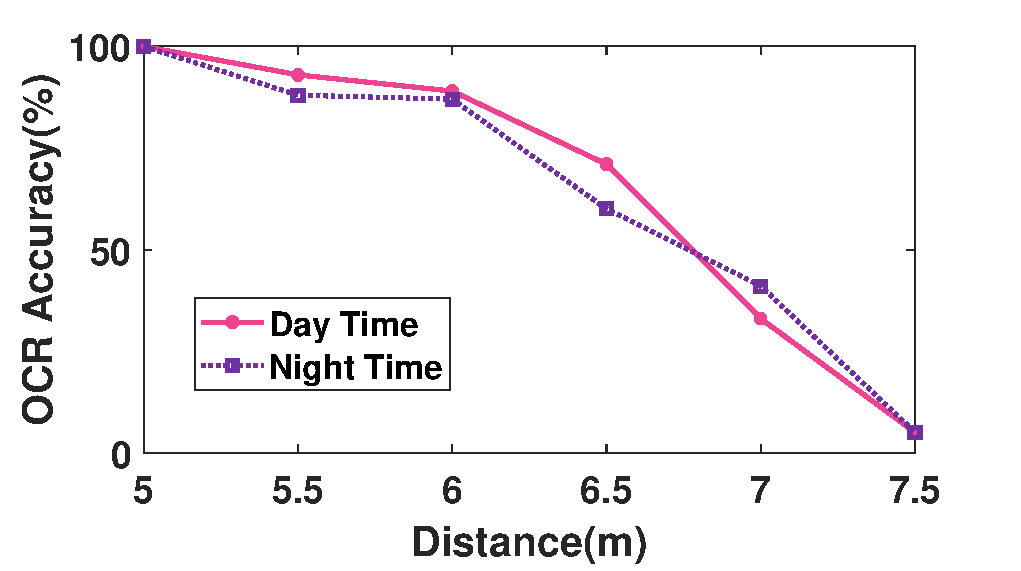
\includegraphics[width=0.24\textwidth]{./pic/data_2_2.pdf}\label{fig-random-2}}
%     \hfill
%     \caption{Performance in Controlled Environment (a,b) and Random Environment (c,d).}
%     \label{fig-performance-1}
% \end{figure*}
We evaluate the performance of the network model in different training and testing conditions. We perform the following experiments with two COTS smartphones: a Redmi 6A smartphone, with a single rear camera with 13 million pixels and digital zoom only, and a HUAWEI P40 Pro, with multiple rear cameras. The telephoto camera possesss up to 5x optical zooming ability which we will utilize fully in our experiments.
 
\subsection{Performance In Controlled Environments}
In these experiments, we train and test the model with the images captured with exactly the same environment parameters, and used Peak Signal to Noise Ratio to evaluate the accuracy of the recovered images. The results are shown in Figure~\ref{fig-control-1} and Figure~\ref{fig-control-2}. Moreover, the ultimate goal of our system is the readability of the recovered images, so we also used Optical Character Recognition(OCR) services to evaluate the accuracy. The model with traditional lens without optical zoom(hereafter refered as traditional lens) is trained and tested at 1-2 meters range, while the lens with optical zoom(hereafter refered as optical lens) at 5-7.5 meters, at which distance less than 5\% of the characters (only the simplest ones) can be recognized by humans from the photos without the assistance of SR algorithms. The PSNR and OCR results are shown in Fig. ~\ref{fig-control-1}.

This model can achieve an OCR accuracy above 90\% at 1.8m with traditional lens in both day and night time. The PSNR is higher than 10 as well. OCR accuracy and PSNR drops in night time since the darker environmental lighting condition as well as with the increasing of distance since the longer distance means more blurs. For Figure~\ref{fig-control-2}, we can see the OCR accuracy is larger than 90\% at 6m with optical lens. The performance is relatively consistent in both day and night time. Considering the complexity of Chinese characters, and the assist of context when read by an OCR recognizer, we believe this level of accuracy can provide sufficient data at a shoulder surfing scenario, thus proving the efficiency of our model.
\begin{figure}[!t]
    \centering
    \subfigure[Traditional Lens]{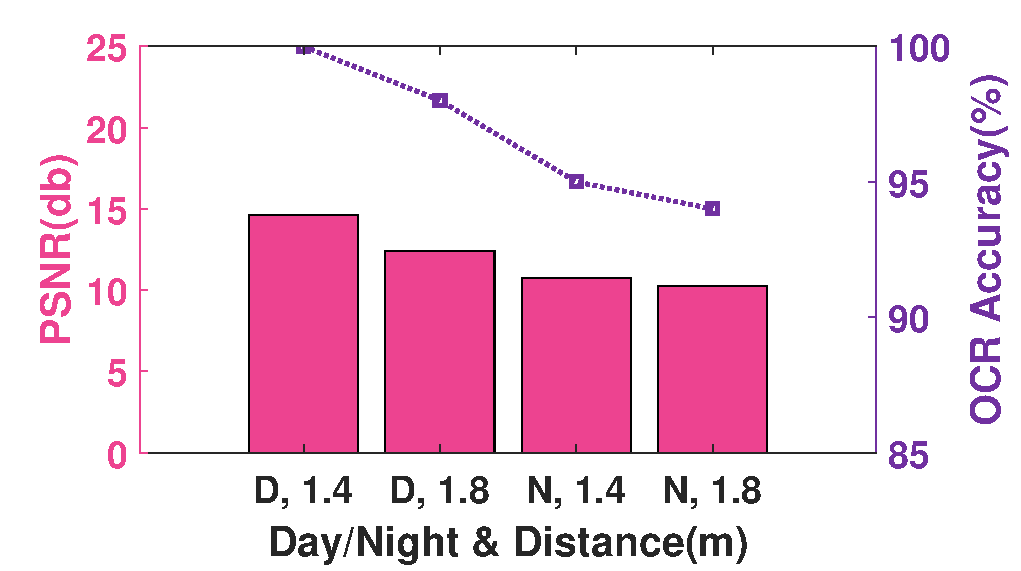
\includegraphics[width=0.36\textwidth]{./pic/data_1.pdf}\label{fig-control-1}}
    \subfigure[Optical Lens]{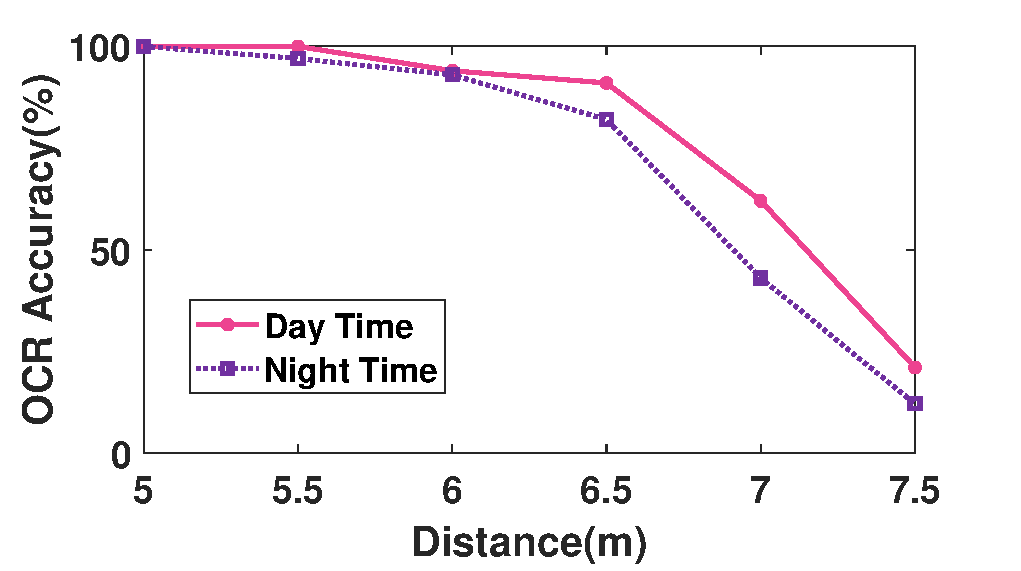
\includegraphics[width=0.36\textwidth]{./pic/data_1_2.pdf}\label{fig-control-2}}
    \hfill
    \caption{Performance in Controlled Environment using Traditional Lens and Optical Lens.}
    \label{fig:control}
\end{figure}

In the optical zoom group, the accuracy of the model dropped drastically at 7m distance. Increased distances means less data and less restrictions of the possible outputs, which leads to artifacts(missing or misplaced strokes, etc.). It is the nature of Chinese characters that one mistaken stroke will largely affect its readability, leading to the result that while the pixel-wise error rises steadily with the increased distance, the accuracy will experience a drastic drop.

\subsection{Performance In Random Environments}
We train the model with data captured in different environments, as mentioned before, and test its ability in other environments. The results are shown in Figure~\ref{fig-random-1} and Figure~\ref{fig-random-2}. For Figure~\ref{fig-random-1}, the model can still achieve an OCR accuracy above 85\% at 1.8m with traditional lens. From Figure~\ref{fig-random-2}, the OCR accuracy keeps higher than 90\% at 6m with optical lens. This verifies the efficiency of our model for environment adaption.
 
\begin{figure}[!t]
    \centering
    \subfigure[Traditional Lens]{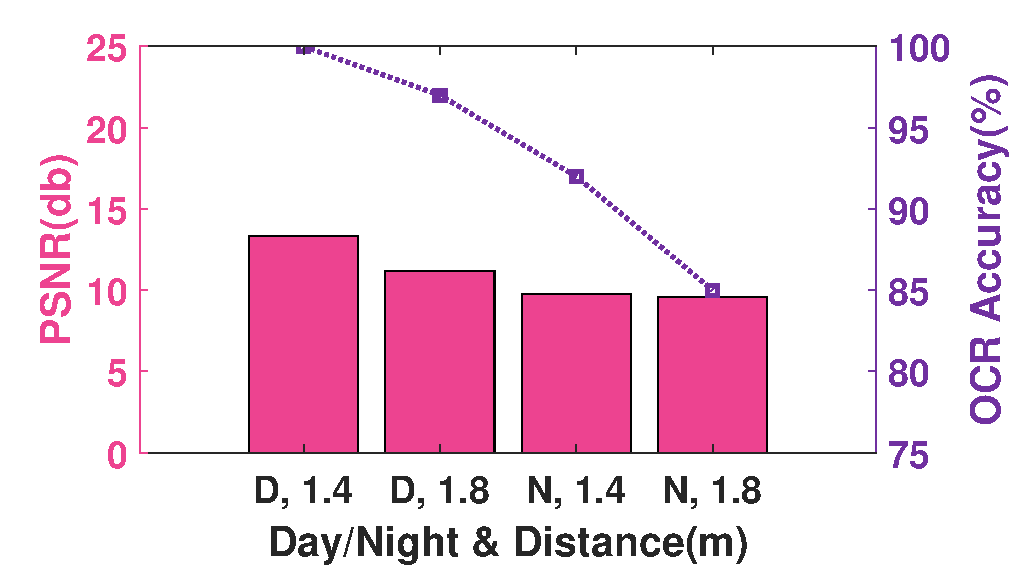
\includegraphics[width=0.36\textwidth]{./pic/data_2.pdf}\label{fig-random-1}}
    \subfigure[Optical Lens]{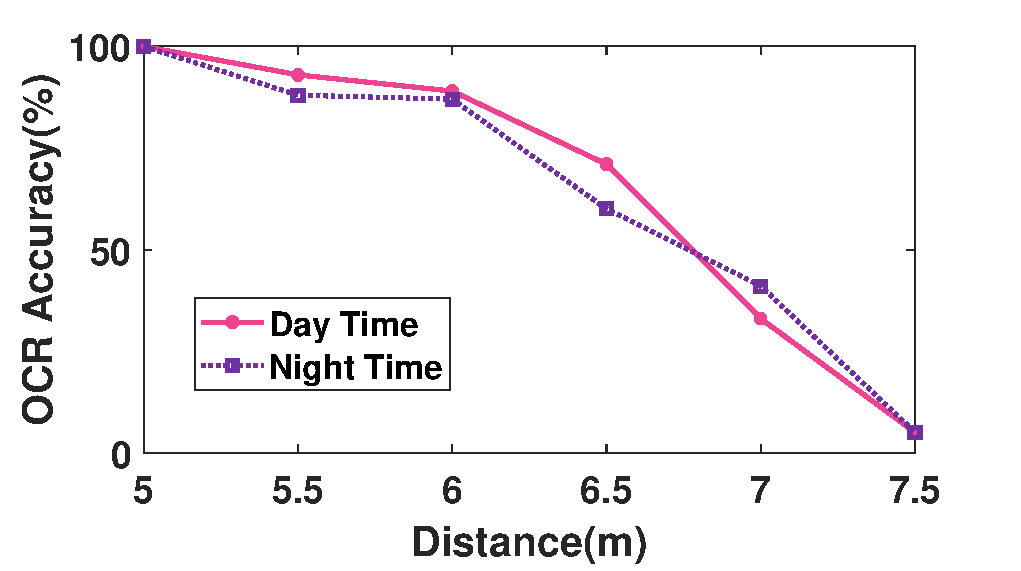
\includegraphics[width=0.36\textwidth]{./pic/data_2_2.pdf}\label{fig-random-2}}
    \hfill
    \caption{Performance in Random Environment using Traditional Lens and Optical Lens.}
    \label{fig:control}
\end{figure}

We compare the results to discover the influence of the surrounding environment: The model performs best in daytime and weaker illumination may decrease its ability. Also, the model performs better at closer distances. As the model is trained initially on the 5m group data, it performs especially well at this distance, while the accuracy at other distances experience certain levels of decrease. Also, similar to the experiments at controlled environments, random artifacts start to encompass OCR compensation, rendering the result images highly unreadable, until at 7.5m distance only the simplest characters can escape from being flooded by noise.

% \begin{figure*}[!t]
%     \centering
%     \subfigure[Traditional Lens]{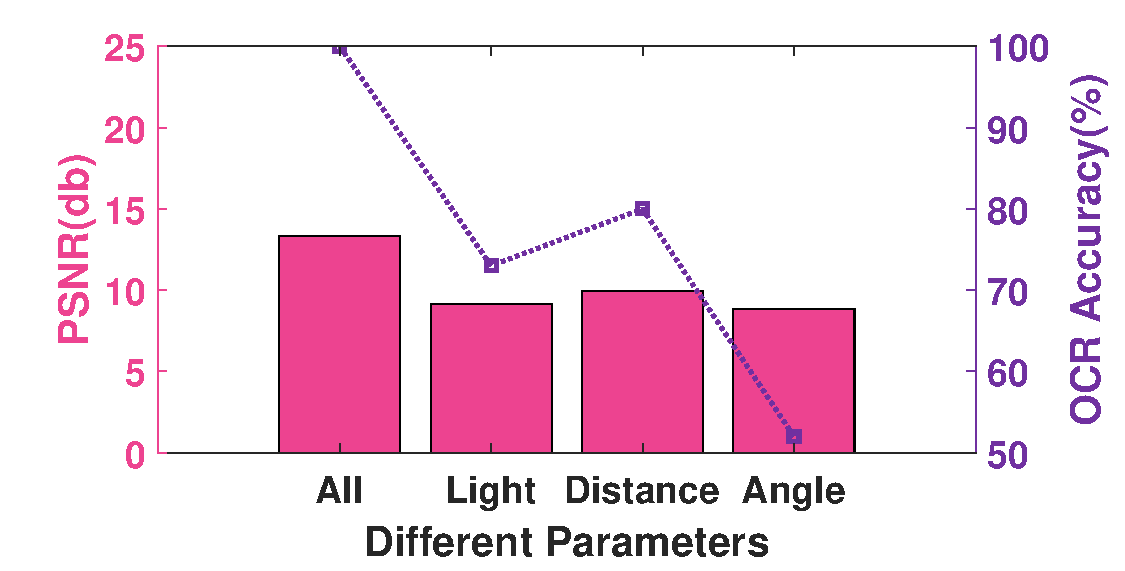
\includegraphics[width=0.24\textwidth]{./pic/data_3.pdf}\label{fig-adapt-tranditional}}
%     \subfigure[Optical Lens]{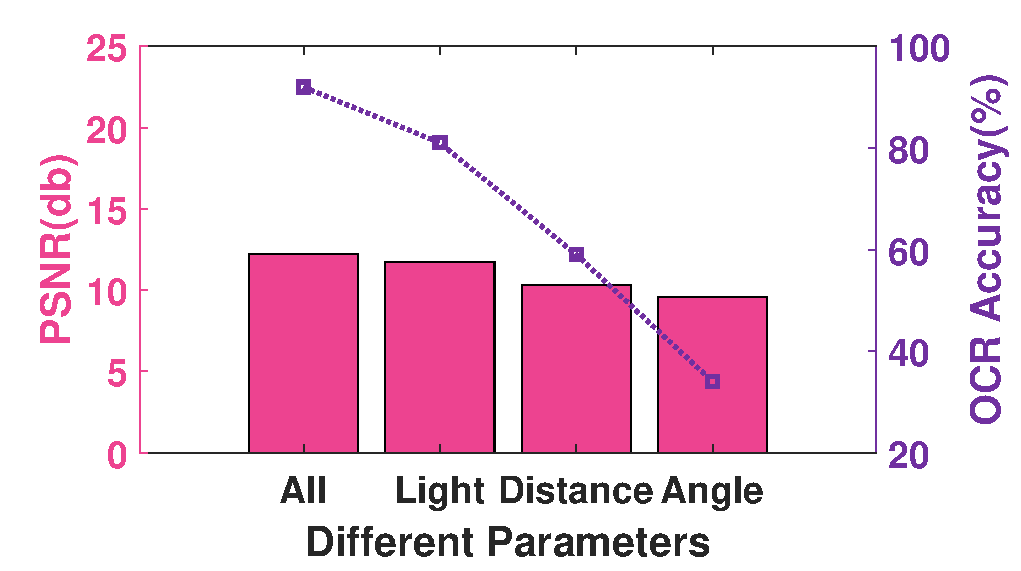
\includegraphics[width=0.24\textwidth]{./pic/data_4.pdf}\label{fig-adapt-optical}}
%     \subfigure[Traditional Lens]{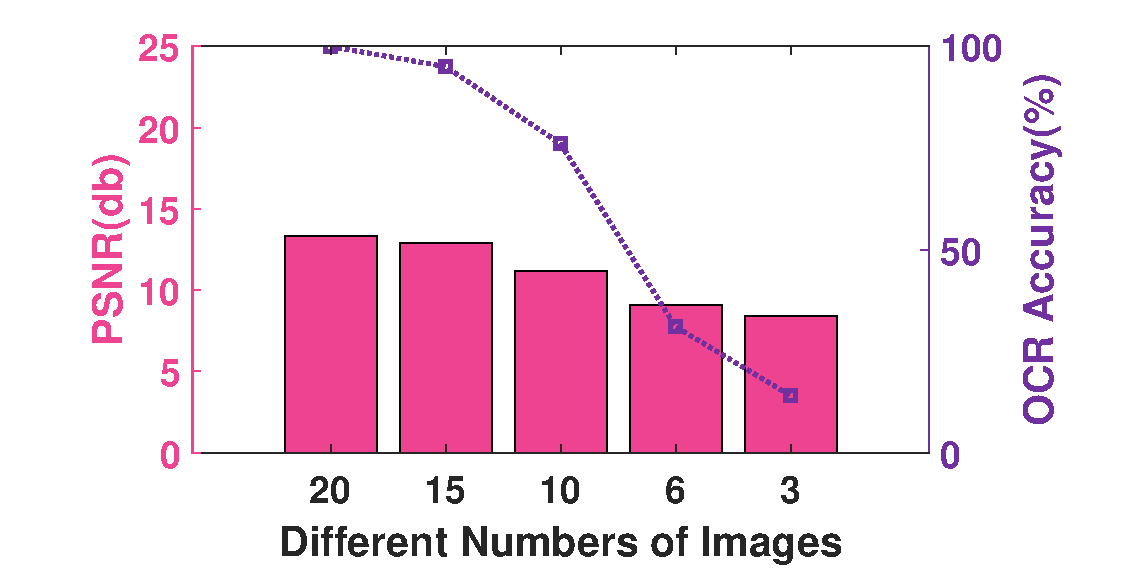
\includegraphics[width=0.24\textwidth]{./pic/data_5.pdf}\label{fig-image-tranditional-2}}
%     \subfigure[Optical Lens]{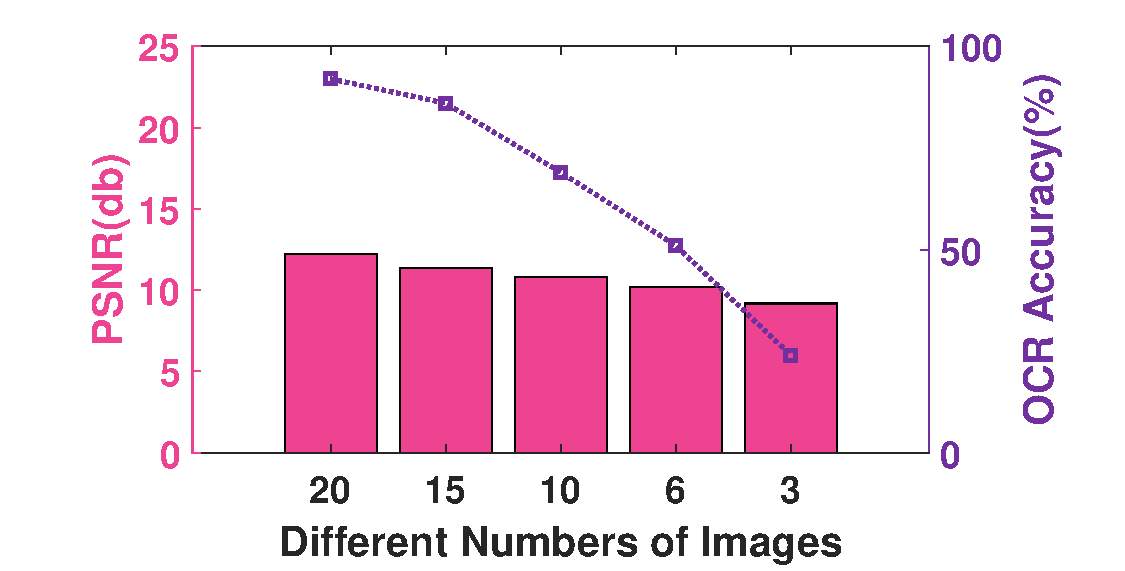
\includegraphics[width=0.24\textwidth]{./pic/data_6.pdf}\label{fig-image-optical-2}}
%     \hfill
%     \caption{Performance for Adapting Ability and various processing images.}
%     \label{fig:adapting}
% \end{figure*}


\subsection{Performance with fewer avaliable images}
\begin{figure}[!t]
    \centering
    \subfigure[Traditional Lens]{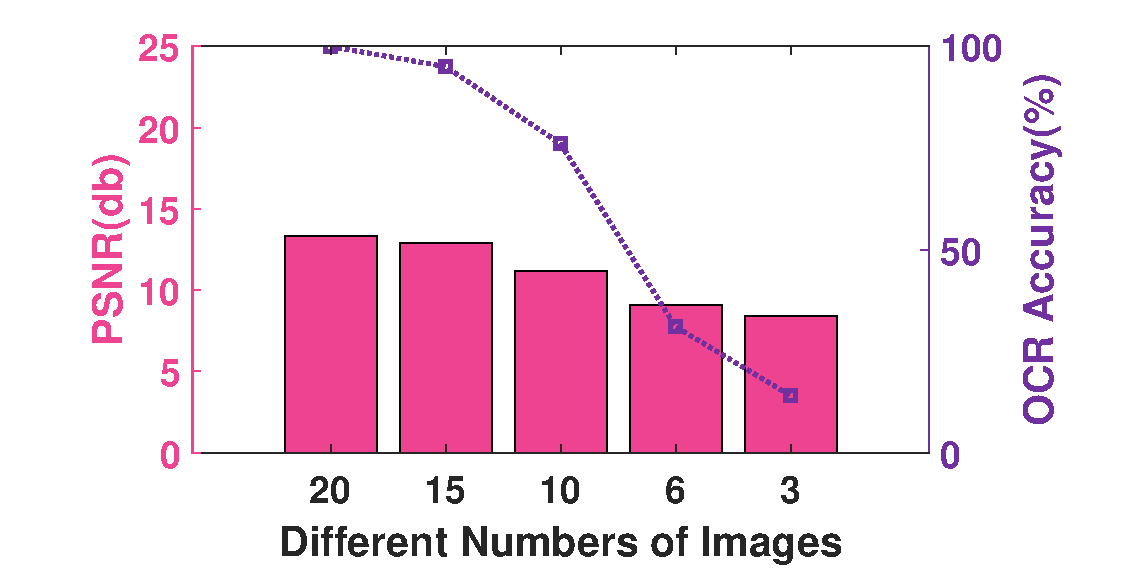
\includegraphics[width=0.36\textwidth]{./pic/data_5.pdf}\label{fig-image-tranditional-2}}
    \subfigure[Optical Lens]{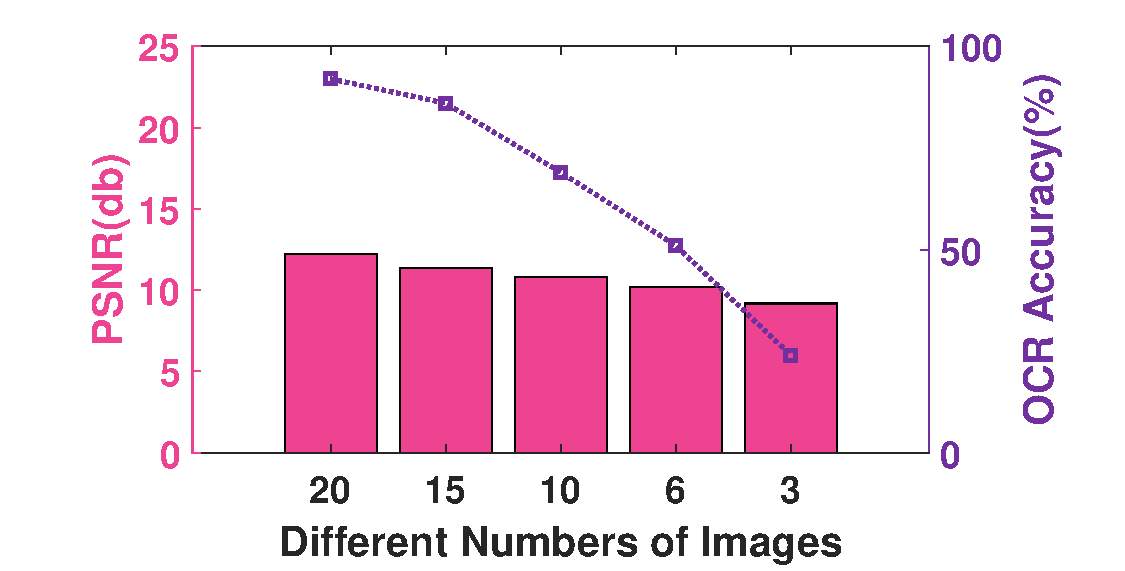
\includegraphics[width=0.36\textwidth]{./pic/data_6.pdf}\label{fig-image-optical-2}}
    \hfill
    \caption{Performance with fewer avaliable images using Traditional Lens and Optical Lens.}
    \label{fig:number}
\end{figure}
As mentioned in sec.~\ref{sec-design}, our model is designed to work on any number of input images, the only limitation being that these images are snapshots of the same scene. This design is requisite because in certain scenraios the data displayed on the victim's screen is transient and ever-changing, e.g. password entry, where only the last character of the password is visible. We evaluated the impact of fewer avaliable images to the performance of the SR model. The results are shown in fig.~\ref{fig:number}. We tested at the 1.8m daytime scenario for traditional lens and 6m daytime scenario for optical lens.

In the tradition lens group the performance of the model drops dramatically with fewer than 10 images, indicating that not enough input information is avaliable to rule out all possibilities of the displayed characters. The optical lens group displayed a steady decent of accuracy when fewer images are avaliable, which is expected, as the blur patterns are more complex and the differences between frames more pronounced, so that the images are more precious to the model and contain less overlapping data, and removing any of them will cause losses in accuracy.

\subsection{Adapting Ability}
We train the model with fewer groups of data, exposing it to fewer variations of environment parameters, and examine the model's performance in other environments. The results are shown in Figure~\ref{fig:adapting}.

\begin{figure}[!t]
    \centering
    \subfigure[Traditional Lens]{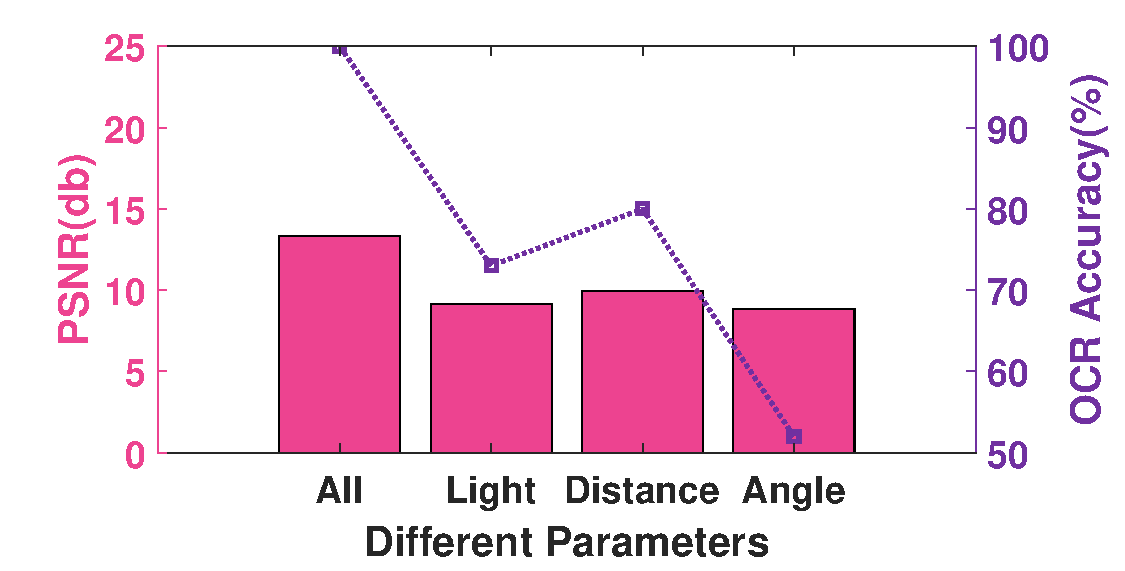
\includegraphics[width=0.36\textwidth]{./pic/data_3.pdf}\label{fig-adapt-tranditional}}
    \subfigure{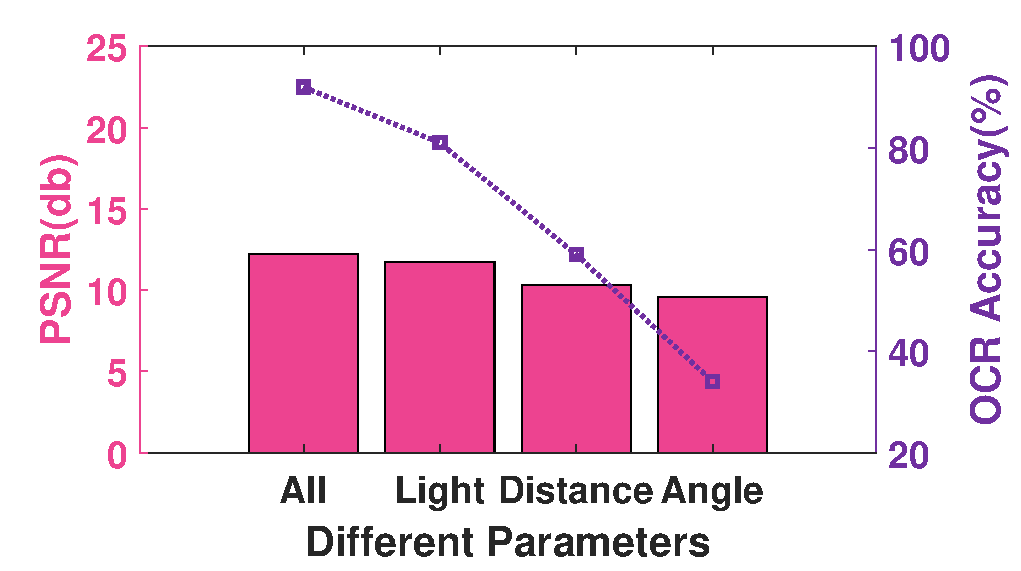
\includegraphics[width=0.36\textwidth]{./pic/data_4.pdf}\label{fig-adapt-optical}}
    \hfill
    \caption[Optical Lens]{Performance for Adapting Ability using Traditional Lens and Optical Lens.}
    \label{fig:adapting}
\end{figure}

We observed that variations in light and angle parameter in training data is crucial to a robust model. Variations in distance is not so influential to the results, given that the distances are between 1 and 2 meters. Distance changes do not have such a large impact on the size of the characters shown in the images, so that features extracted from a fixed distance might still exist when these characters vary slightly in size. However, if the network is not exposed to angled images during the training process, the rotations and deformations caused by these angles will easily disturb the feature extraction process.

\subsection{Comparison with other architectures}
We train and test other commonly used architectures with the same sets of data and evaluate their results. We chose SRCNN, a commonly used single image SR network, and applied it to each single image before merging the results by pixel-level average. We also used a multi-frame version of CNN consisting of 3D convolutional layers, designed for video super resolution(VideoSR). However, as mentioned above, it is very difficult for the single image approaches to utilize information and distinguish the noisy and deformed patterns, while VideoSR approaches rely upon consistency between frames, so they fail to give satisfactory results. We used the relatively easy 'daytime 1.2m-distance direct with traditional lens' group of data for testing. The results are shown in Table~\ref{table-comp}.
\begin{table}[!t]
    \centering
    \caption{Comparison with existing systems.}
    \begin{tabular}{@{}cccc@{}}
        \toprule
    System & SRPeek & SRCNN & VideoSR \\ \midrule
    PSNR(db) & 13.32 & 7.69 & 8.403\\ 
    OCR Accuracy(\%) & 100 & 10 & 23\\ \bottomrule
    \end{tabular}
    \label{table-comp}
\end{table}

We can see that the PSNR of SRPeek is 13.32dB which 73.2\% and 58.6\% larger than that of SRCNN and VideoSR. For the OCR accuracy, SRPeek can recognize all characters, but SRCNN and VideoSR can only recognize 10\% and 23\% of them. The results show the efficiency of our SR model in comparison with existing models.

% \section{System Evaluation}
\section{Case Study}
\subsection{Accuracy}
We build the system on smartphone and evaluate its performance in real-life environments. We experiment with a Redmi 6A smartphone (with a camera of 13 million pixels) for the attacker and a HUAWEI Mate8 smartphone for the victim. As the telephoto cameras can assist the attacker to see clearly at approximately 3m distance without any aid from SR algorithms, we believe it is insignificant to further extend this distance to judge it as a threat to privacy, so that the following experiments are performed with traditional lens at 1-2m range. We ask 5 human participants to read the reconstructed characters to evaluate the usability of our model. No participants can read the unprocessed images, but all of them can decipher the information on the reconstructed image without much difficulty. The results are shown in Table~\ref{table-scenarios}.

The results show that Human can read 95\%, 85\% and 70\% contents in home, transport and theater while the OCR accuracy is 100\%, 10\% and 23\%. That verifies human can obtain the most parts of informations from the peeking in various environments. In transport, the vibration of smartphone and the darker environment can fool the OCR model for content recognition in comparison with human recognition so that leads lower accuracy in transport and theater.

\begin{table}[!t]
    \centering
    \caption{Recognition accuracy in various scenarios.}
    \begin{tabular}{@{}cccc@{}}
        \toprule
    Scenarios & Home & Transport & Theater \\ \midrule
    Baseline & 5 & 0 & 0\\ 
    \midrule
    OCR & 100 & 10 & 23\\ 
    Human & 95 & 85 & 70\\ \bottomrule
    \end{tabular}
    \label{table-scenarios}
\end{table}

\subsection{Influence of hand tremors}
We ask 5 participants to capture images with handheld smartphones, keeping their hand still to their greatest effort(Handheld camera). We process these images and let them read the results. We compare this performance to the data collected on stationary phones to evaluate the influence of hand tremors.
We also ask participants to hold a smartphone in their hands and read a piece of text, without other additional instructions(Handheld target). The user may freely interact with the phone when reading. We capture images of the phone at the same time to see how our system deal with a moving target screen.The results are shown in Table~\ref{table-tremor}.

\begin{table}[!t] 
    \centering
    \caption{Impact of hand tremors when the camera(attacker phone) and/or target(victim phone) is handheld.}
    \begin{tabular}{ccccc}
        \toprule
    Items & None & Camera & Target & Both  \\
    \midrule
    Baseline & 5 & 0 & 5& 5\\ 
    \midrule
    OCR & 95 & 85 & 80 & 80\\ 
    Human & 95 & 85 & 80 & 85\\ \bottomrule
    \end{tabular}
    \label{table-tremor}
\end{table}

We can see when tremors happen, the recognition accuracy drops from 95\% to 85\%/80\% for both OCR tools and human. We conclude from the results that hand tremors can impact the performance of our system. Although the edges of the phone are notable marks for image alignment, small shifts in the sub-pixel level will cause blurriness in the results of the networks, lowering the readability of the outputs. 


\subsection{Success rate in different tasks}
We test the success rate of obtaining crucial information when the observed participant perform several tasks on a phone: reading text message, typing text message, entering PIN, and typing password with numbers, English and special characters. The observed participant will turn off the screen of his phone as soon as he/she finishes the task, while the observing participant will observe through our APP, constantly capturing images and processing them to display a real-time and magnified view of the observed phone. For the first two tasks, we ask the observing participant several questions to test if he/she have collected the vital information(e.g. the name or the location mentioned in the text). For the task of recognizing PIN and passwords, we use accuracy per character as a supplementary evaluation metric. In these two scenarios, we ignore the virtual keyboard and view only the textbox, assuming that the last character of the entered string is always visible. Fewer photos will be available for each character but decipfering English characters is also easier than Chinese characters, and we trained a model specifically for each task(with the same neural network architecture), the training images containing only English characters and numbers(or only numbers for the PIN entry scenario). The results are shown in Table~\ref{table-task}.

\begin{table}[!t]
\centering
\caption{Success rate in different tasks.}
\label{table-task}
\begin{tabular}{@{}ccccc@{}}
	\toprule
Accuracy & Read text & Type text & Enter PIN & Enter password\\ \midrule
Raw Image & 5 & 0 & 0 & 0\\
SRPeek & 100 & 100 & 100 & 80\\ \bottomrule
\end{tabular}

\end{table}

We prove from this experiment that our system functions normally in everyday scenarios and poses a threat to screen privacy.

\subsection{Perceived shoulder surfing susceptibility}
We ask the observed participant to rate the perceived shoulder-surfing susceptibility in these scenario. The attacker will be sitting or standing behind the participant at 1.8m range, pretending to be interacting with their own phone while continuously running the shoulder-surfing APP. None of the participants were alerted by the attacker's behavior and reported suspicion of shoulder-surfing. We believe that our system can enable a malicious attacker to gather large amounts of critical information from the victim while remaining unnoticed.




